\section{Einführung}
\subsection{Analog/Digital}
Signale werden quantisiert (Analoges Signal auf Digitales Raster umgewandelt).\\
\noindent\textbf{Nyquist-Shannon Abtasttheorem} besagt, dass $f_{abtast} > 2 \cdot f_{sigmax}$, damit Ursprungssignal rekonstruiert werden kann. \textbf{Dynamischer Bereich} eines AD-Wandlers ist ungefähr $DR_{ADC} \approx \frac{U_{max}}{U_{min}}$. (Fastformel $DR_{ADC}[dB] \approx 6 \cdot \#Bit$)

\begin{minipage}{\textwidth}
	\noindent\textbf{KKNF} - Kanonische konjunktive Normalform\\
	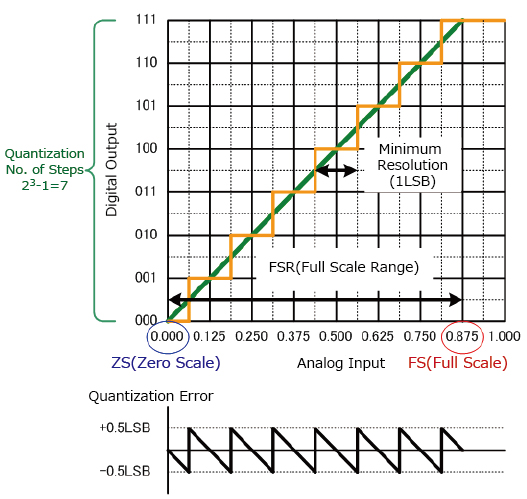
\includegraphics[height=20em]{./Images/ADC.jpg}
\end{minipage}


\noindent\textbf{Warum Digital?} 
Einfacher im Design $\bullet$ Einfacher im Test $\bullet$  Reproduzierbar in Herstellung  $\bullet$ Störsicherer
\\ \\
\noindent\textbf{Warum Analog?}
Interface zu realen Welt ist immer Analog $\bullet$ Instantane Resultate möglich

\subsection{Zahlensystem}
\subsubsection{Begriffe}
Das \textbf{Nibble} ist eine Binärzahl in Gruppen von 4 Bits. \textit{z.B. 0111 1001}. \\
\noindent
Most Significant Bit (\textbf{MSB}) Bit mit höchster Wertigkeit steht links. \\
\noindent
Least Significant Bit (\textbf{LSB}) Bit mit tiefster Wertigkeit steht rechts.

\subsubsection{Umwandlung}
Dezimal $109.78125_{(10)}$ $\rightarrow$ Binär \textit{$110'1101.1100'1_{(2)}$} \\
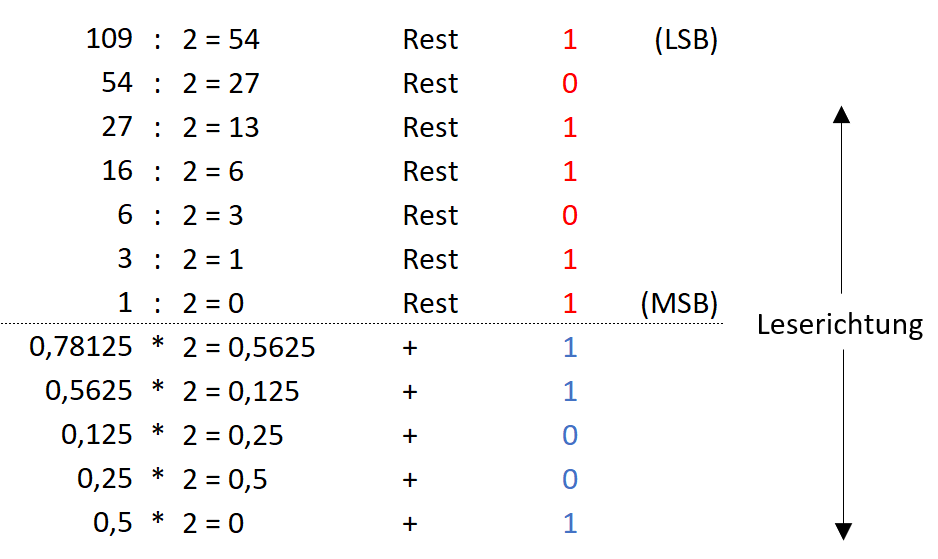
\includegraphics[width=\columnwidth]{./Images/Umwandlung.png}

\noindent
Abbruchkriterium
\begin{itemize}[nosep]
	\item Resultat wird 0
	\item Bruch wiederholt sich periodisch
	\item Resultat hat erforderliche Stellen
\end{itemize}

\subsubsection{Dualsystem}
\noindent\textbf{Vorzeichendarstellung}:
Hat den Nachteil, dass $\pm0$ verfügbar ist und Subtraktion funktioniert nicht. \\ \\
\noindent\textbf{Einerkomplement}:
Hat den Nachteil, dass $\pm0$ verfügbar ist (Umwandlung durch Invertieren):. 
\\ \\
\noindent\textbf{Zweierkomplement}: Keine Nachteile.
Beispiel (Umwandlung durch Invertieren und + 1):
\begin{align*}
	5 &\rightarrow -5 \\
	0101 &\rightarrow 1011
\end{align*}

\noindent Der \textbf{Wertebereich} kann mit $-2^{n-1} \dots 0 \dots 2^{n-1}-1$ (n: Anzahl Bits) ermittelt werden.


\subsubsection{Arithmetik}
Die Binäre-\textbf{Addition} funktioniert identisch zum Dezimalsystem. Bei der Subtraktion wird der Übertrag ignoriert:
\begin{center}
	\begin{tabular}{r|ccccc}
		$4_{10}$ & & 0 & 1 & 0 & 0 \\
		$-3_{10}$ & & 1 & 1 & 0 & 1 \\
		\hline
		\tiny{Borrow} & \textcolor{red}{\tiny{1}} & \textcolor{red}{\tiny{1}} & \tiny{0} & \tiny{0} & \\
		\hline
		=     &  & 0 & 0 & 0 & 1 \\
		\hhline{======}
	\end{tabular}
\end{center}

\noindent Das Borrow $n$ und $n-1$ zeigt an, ob das Ergebnis korrekt ist, oder ein Überlauf statt gefunden hat.

\begin{center}
	\begin{tabular}{rc|c}
		& \textbf{Korrekt} & \textbf{Überlauf} \\
		\hline
		A + B & $c_n = 0,c_{n-1}=0$ & $c_n = 0,c_{n-1}=1$ \\
		A - B & $c_n = c_{n-1}$ & \textit{Nicht möglich }\\
		-A - B & $c_n = 1,c_{n-1}=1$ & $c_n = 1,c_{n-1}=0$ \\
	\end{tabular}
\end{center}

\noindent Auch bei der Binäre \textbf{Multiplikation} kann das Dezimalsystem verwendet werden:

\begin{center}
	\begin{tabular}{r|cccccccccc}
		$10_{10} \cdot 11_{10}$ & & 1 & 0 & 1 & 0 & $\times$ & \textcolor{orange}{1} & \textcolor{green}{0} & \textcolor{blue}{1} & \textcolor{red}{1} \\
		\hline
		                        + & &   &   &   &   &  & \textcolor{red}{1} & \textcolor{red}{0} & \textcolor{red}{1} & \textcolor{red}{0} \\
					            + & &   &   &   &   &  \textcolor{blue}{1} & \textcolor{blue}{0} & \textcolor{blue}{1} & \textcolor{blue}{0} & \\
     	                         + & &   &   &   &   \textcolor{green}{0} & \textcolor{green}{0} & \textcolor{green}{0} & \textcolor{green}{0} & & \\
					            + & &   &   &   \textcolor{orange}{1} & \textcolor{orange}{0} & \textcolor{orange}{1} & \textcolor{orange}{0} & & & \\
		\hline
		\tiny{Carry}            & &   &   &  \tiny{0} & \tiny{1} & \tiny{0} & \tiny{0} & \tiny{0} & \tiny{0} & \\
		\hline
		$110_{10}$                       & &   &   &  1 & 1 & 0 & 1 & 1 & 1 & 0 \\
		\hhline{===========}
	\end{tabular}
\end{center}
